\begin{figure*}[hb]
  \centering

  \begin{subfigure}[t]{0.42\tw}\centering
    \includegraphics[width=\textwidth]{no-revocation.svg.pdf}
    \caption{Stock Mesos -- No Revocation}
    \label{fig:wo-revocation}
  \end{subfigure}%
  \hfill
  \begin{subfigure}[t]{0.42\tw}\centering
    \includegraphics[width=\textwidth]{revocation.svg.pdf}
    \caption{Mesos With Revocation}
    \label{fig:w-revocation}
  \end{subfigure}%

  \caption{\textbf{Comparison of Mesos With and Without Revocation Enabled}
  Example Mesos cluster with two slots. Both example frameworks have two parallel tasks so they are able
  to fully utilize the entire cluster. Framework 2 arrives later than the Framework 1. Yellow bars
  corrrespond to the time that the framework has to wait for an offer from Mesos. Red bar corresponds
  to the time that framework is running a task on a node.
  }
  \label{fig:revocation}
\end{figure*}
